

\tikzset{every picture/.style={line width=0.75pt}} %set default line width to 0.75pt        

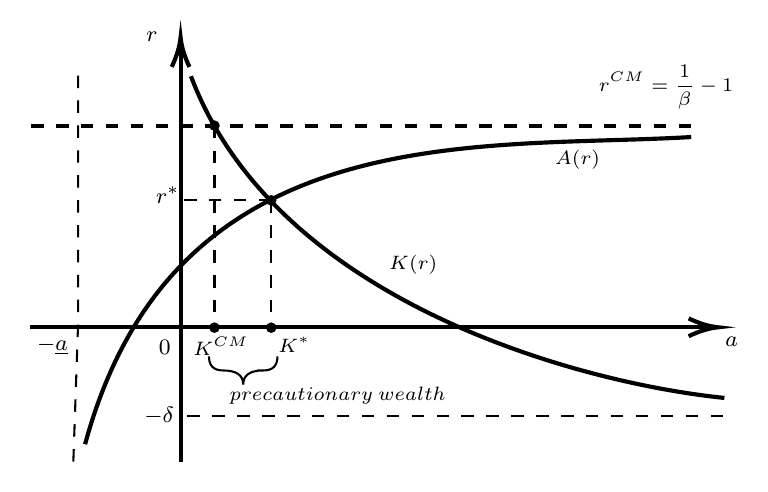
\begin{tikzpicture}[x=0.75pt,y=0.75pt,yscale=-1,xscale=1]
%uncomment if require: \path (0,326); %set diagram left start at 0, and has height of 326

%Straight Lines [id:da003982959695679522] 
\draw [line width=1.5]    (113.33,222) -- (442,222) ;
\draw [shift={(445,222)}, rotate = 180] [color={rgb, 255:red, 0; green, 0; blue, 0 }  ][line width=1.5]    (14.21,-4.28) .. controls (9.04,-1.82) and (4.3,-0.39) .. (0,0) .. controls (4.3,0.39) and (9.04,1.82) .. (14.21,4.28)   ;
%Straight Lines [id:da4435949040681568] 
\draw [line width=1.5]    (186,287) -- (186,85.33) ;
\draw [shift={(186,82.33)}, rotate = 90] [color={rgb, 255:red, 0; green, 0; blue, 0 }  ][line width=1.5]    (14.21,-4.28) .. controls (9.04,-1.82) and (4.3,-0.39) .. (0,0) .. controls (4.3,0.39) and (9.04,1.82) .. (14.21,4.28)   ;
%Curve Lines [id:da004845910574244883] 
\draw [color={rgb, 255:red, 0; green, 0; blue, 0  }  ,draw opacity=1 ][line width=1.5]    (140,278.33) .. controls (183,119.33) and (330,136.33) .. (432,130.33) ;
%Straight Lines [id:da20885399252750636] 
\draw [dash pattern={on 4.5pt off 4.5pt},color={rgb, 255:red, 0; green, 0; blue, 0 }  ,draw opacity=1 ][line width=1.5]    (114,125) -- (437,125) ;
%Straight Lines [id:da4890932186968713] 
\draw [line width=0.75]  [dash pattern={on 4.5pt off 4.5pt}]  (134.33,286.67) -- (136.67,218.67) -- (136.67,97.98) ;
%Straight Lines [id:da16192855911262694] 
\draw  [dash pattern={on 4.5pt off 4.5pt}]  (202.33,124.83) -- (202.33,222.17) ;
\draw [shift={(202.33,222.17)}, rotate = 90] [color={rgb, 255:red, 0; green, 0; blue, 0 }  ][fill={rgb, 255:red, 0; green, 0; blue, 0 }  ][line width=0.75]      (0, 0) circle [x radius= 2.01, y radius= 2.01]   ;
\draw [shift={(202.33,124.83)}, rotate = 90] [color={rgb, 255:red, 0; green, 0; blue, 0 }  ][fill={rgb, 255:red, 0; green, 0; blue, 0 }  ][line width=0.75]      (0, 0) circle [x radius= 2.01, y radius= 2.01]   ;
%Curve Lines [id:da1965108414386998] 
\draw [color={rgb, 255:red, 0; green, 0; blue, 0 }  ,draw opacity=1 ][line width=1.5]    (191,101.02) .. controls (232,210.02) and (379,249.02) .. (448,256.02) ;
%Straight Lines [id:da7694531923876664] 
\draw  [dash pattern={on 4.5pt off 4.5pt}]  (447.33,264.83) -- (186,264.83) ;
%Straight Lines [id:da842562709955549] 
\draw  [dash pattern={on 4.5pt off 4.5pt}]  (229.67,160.83) -- (229.67,222.17) ;
\draw [shift={(229.67,222.17)}, rotate = 90] [color={rgb, 255:red, 0; green, 0; blue, 0 }  ][fill={rgb, 255:red, 0; green, 0; blue, 0 }  ][line width=0.75]      (0, 0) circle [x radius= 2.01, y radius= 2.01]   ;
\draw [shift={(229.67,160.83)}, rotate = 90] [color={rgb, 255:red, 0; green, 0; blue, 0 }  ][fill={rgb, 255:red, 0; green, 0; blue, 0 }  ][line width=0.75]      (0, 0) circle [x radius= 2.01, y radius= 2.01]   ;
%Straight Lines [id:da9792716174268414] 
\draw  [dash pattern={on 4.5pt off 4.5pt}]  (229.67,160.83) -- (186,160.83) ;
%Shape: Brace [id:dp53072780230569] 
\draw   (199.67,236) .. controls (199.67,240.53) and (201.93,242.79) .. (206.46,242.79) -- (206.46,242.79) .. controls (212.93,242.79) and (216.17,245.06) .. (216.17,249.59) .. controls (216.17,245.06) and (219.4,242.79) .. (225.87,242.79)(222.96,242.79) -- (225.87,242.79) .. controls (230.4,242.79) and (232.67,240.53) .. (232.67,236) ;

% Text Node
\draw (365,135) node [anchor=north west][inner sep=0.75pt]  [font=\scriptsize,color={rgb, 255:red, 0; green, 0; blue, 0  }  ,opacity=1 ] [align=left] {$\displaystyle A( r)$};
% Text Node
\draw (168,78.14) node [anchor=north west][inner sep=0.75pt]  [font=\footnotesize] [align=left] {$\displaystyle r$};
% Text Node
\draw (386,94) node [anchor=north west][inner sep=0.75pt]  [font=\scriptsize,color={rgb, 255:red, 0; green, 0; blue, 0 }  ,opacity=1 ] [align=left] {$\displaystyle r^{CM} =\frac{1}{\beta } -1$};
% Text Node
\draw (115.33,225) node [anchor=north west][inner sep=0.75pt]  [font=\footnotesize] [align=left] {$\displaystyle -\underline{a}$};
% Text Node
\draw (174,226.66) node [anchor=north west][inner sep=0.75pt]  [font=\footnotesize] [align=left] {$\displaystyle 0$};
% Text Node
\draw (447,225) node [anchor=north west][inner sep=0.75pt]  [font=\footnotesize] [align=left] {$\displaystyle a$};
% Text Node
\draw (167,259) node [anchor=north west][inner sep=0.75pt]  [font=\footnotesize] [align=left] {$\displaystyle -\delta $};
% Text Node
\draw (172.67,152.8) node [anchor=north west][inner sep=0.75pt]  [font=\footnotesize] [align=left] {$\displaystyle r^{*}$};
% Text Node
\draw (285,185.67) node [anchor=north west][inner sep=0.75pt]  [font=\scriptsize,color={rgb, 255:red, 0; green, 0; blue, 0 }  ,opacity=1 ] [align=left] {$\displaystyle K( r)$};
% Text Node
\draw (190.67,225) node [anchor=north west][inner sep=0.75pt]  [font=\scriptsize,color={rgb, 255:red, 0; green, 0; blue, 0 }  ,opacity=1 ] [align=left] {$\displaystyle K^{CM}$};
% Text Node
\draw (231.67,225) node [anchor=north west][inner sep=0.75pt]  [font=\scriptsize,color={rgb, 255:red, 0; green, 0; blue, 0 }  ,opacity=1 ] [align=left] {$\displaystyle K^{*}$};
% Text Node
\draw (255,255) node  [font=\scriptsize] [align=left] {\begin{minipage}[lt]{68pt}\setlength\topsep{0pt}
$\displaystyle precautionary\ wealth$
\end{minipage}};


\end{tikzpicture}